%&format -translate-file pdf
\documentclass{article}
\usepackage{graphicx}
\usepackage{listings}
\lstset{basicstyle=\ttfamily\tiny}
\title{Project 3}
\author{RT Hatfield}
\date{19 October 2016}
\begin{document}
\maketitle
\begin{itemize}
    \item Here is my code:
    \begin{lstlisting}
private Double getWeight(int a, int b)
{
    PointF p1 = points.ElementAt(a);
    PointF p2 = points.ElementAt(b);

    double dx = p1.X - p2.X;
    double dy = p1.Y - p2.Y;

    return Math.Sqrt(dx * dx + dy * dy);
}

    

private void solveButton_Clicked()
{
    // we'll run Dijkstra's with a default 

    Stopwatch timer = new Stopwatch();

    double heapResult = Dijkstra(timer, false);
    double heapTime = timer.ElapsedMilliseconds;

    double arrayResult = 0.0;
    double arrayTime = 0.0;

    if (arrayCheckBox.Checked)
    {
        timer.Reset();
        arrayResult = Dijkstra(timer, true);
        arrayTime = timer.ElapsedMilliseconds;
    }

    heapTimeBox.Text = heapTime.ToString();
    arrayTimeBox.Text = arrayTime.ToString();
    differenceBox.Text = (arrayTime - heapTime).ToString();

    if ((heapResult == arrayResult) || (arrayResult == 0))
    {
        pathCostBox.Text = heapResult.ToString();
    }
    else
    {
        pathCostBox.Text = "Heap and array disagree";
    }
    
}

private double Dijkstra(Stopwatch s, Boolean isArray)
{
    /*
    procedure dijkstra(G, l, s)
    Input: Graph G = (V, E), directed or undirected;
            positive edge lengths { le: e ∈ E}; vertex s ∈ V
    Output: For all vertices u reachable from s, dist(u) is set
            to the distance from s to u.
    
    for all u ∈ V :
    dist(u) = ∞
    prev(u) = nil
    dist(s) = 0
    H = makequeue(V)(using dist - values as keys)
            while H is not empty:
                u = deletemin(H)
            for all edges (u, v) ∈ E:
            if dist(v) > dist(u) + l(u, v):
                dist(v) = dist(u) + l(u, v)
                prev(v) = u
                decreasekey(H, v)
*/
    s.Start();
    int numberOfNodes = points.Count;

    PQueue queue;

    if (isArray)
    {
        queue = new AQueue(numberOfNodes);
    }
    else
    {
        queue = new BQueue(numberOfNodes);
    }

    Double[] dist = new Double[numberOfNodes];
    int[] prev = new int[numberOfNodes];

    for (int i = 0; i < numberOfNodes; i++)
    {
        dist[i] = Double.MaxValue;
        prev[i] = -1;
    }

    dist[startNodeIndex] = 0;
    // O(V) if array, O(V log V) if heap
    queue.makeQueue();
    queue.reduceKey(startNodeIndex, 0);

    while(queue.notEmpty())
    {
        // O(V) if array, O(log V) if heap
        int u = queue.deleteMin();

        HashSet<int> E = adjacencyList.ElementAt(u);
        foreach (int v in E)
        {
            Double nextHop = dist[u] + getWeight(u, v);
            if (dist[v] > nextHop)
            {
                dist[v] = nextHop;
                prev[v] = u;
                // O(1) if array, O(log V) if heap
                queue.reduceKey(v, nextHop);
            }
        }
    }

    s.Stop();

    // if it's not an array, go ahead and draw the path
    if (!isArray)
    {

        Pen p = new Pen(Color.Black, 1);
        Font arialFont = new Font("Arial", 11);

        int node = stopNodeIndex;
        int parent = prev[stopNodeIndex];

        while (parent != -1)
        {
            graphics.DrawLine(p, points[node], points[parent]);

            RectangleF rectf = new RectangleF(70, 90, 80, 80);//x, y, width, height
            rectf.X = Math.Abs(points[node].X + points[parent].X) / 2;
            rectf.Y = Math.Abs(points[node].Y + points[parent].Y) / 2;
            graphics.DrawString(((int) getWeight(node, parent)).ToString(), arialFont, Brushes.Black, rectf);

            node = parent;

            parent = prev[parent];

        
        }
    }

    return dist[stopNodeIndex];
}

public class Node
{
    public int pointsIndex;
    public int position;
    public double distance;
    public Node(int ptIndex)
    {
        pointsIndex = ptIndex;
        position = -1;
        distance = 0;
    }
}

public interface PQueue
{
    void makeQueue();
    void reduceKey(int key, Double newVal);
    int deleteMin();
    bool notEmpty();
}

public class BQueue : PQueue
{
    private int parentOf(int node)
    {
        return node / 2;
    }

    private int leftChildOf(int node)
    {
        return 2 * node;
    }

    private int rightChildOf(int node)
    {
        return 2 * node + 1;
    }

    Node[] node_values;
    Double[] weights;
    List<Node> nodes;
    
    int occupied;
    int size;


    public BQueue(int size)
    {
        this.size = size;

        node_values = new Node[size];

        weights = new Double[size];
        nodes = new List<Node>();

        occupied = 0;  // kinda a pointer to last empty space
    }

    // constant time
    void Swap(int position1, int position2)
    {
        Node temp = node_values[position1];
        node_values[position1] = node_values[position2];
        node_values[position2] = temp;
        node_values[position1].position = position1;
        node_values[position2].position = position2;

        Double temp2 = weights[position1];
        weights[position1] = weights[position2];
        weights[position2] = temp2;
    }

    // This is O(log v) in time, as I must reorder part of the tree with 
    // almost all adds, but O(1) in space because it's just one more item
    public void insert(Node item, double priority)
    {
        // Add the item to the heap in the end position of the array 
        //  (i.e. as a leaf of the tree)
        int position = occupied++;
        node_values[position] = item;
        item.position = position;
        weights[position] = priority;
        // Move it upward into position, if necessary
        bubbleUp(position);
        nodes.Add(item);
    }

    void bubbleUp(int position)
    {
        while ((position > 0) && (weights[parentOf(position)] > weights[position]))
        {
            int original_parent_pos = parentOf(position);
            Swap(position, original_parent_pos);
            position = original_parent_pos;
        }
    }

    // O(v log v), running insert v times
    public void makeQueue()
    {
        for (int i = 0; i < size; i++)
        {   
            insert(new Node(i), Double.MaxValue);
        }
    }

    // Time and space are O(log v).  We are rebalancing the whole tree each time.
    public void reduceKey(int key, Double newVal)
    {
        // reduce the key, 
        // then "bubble up" like in insert

        // find and reduce/update key
        int position = nodes[key].position;
        while ((position > 0) && (weights[parentOf(position)] > newVal))
        {
            int original_parent_pos = parentOf(position);
            Swap(original_parent_pos, position);
            position = original_parent_pos;
        }
        weights[position] = newVal;
    }

    // O(log v) because we must rebalance after each deletion
    // Space complexity is constant
    public int deleteMin()
    {
        nodes[node_values[0].pointsIndex].distance = weights[node_values[0].position];
        //data[0].distance = distances[data[0].position];
        Node minNode = node_values[0];
        Swap(0, occupied - 1);
        occupied--;
        siftDown(0);
        return minNode.pointsIndex;
    }

    public bool notEmpty()
    {
        return occupied != 0;
    }

    public void siftDown(int position)
    {
        /*
            *  l ← Left-child-index(i)
            r ← Right-child-index(i)
            if l < heap-size[A] and A[l] > A[i] then
                greatest ← l
            else
                greatest ← i
            end if
            if r < heap-size[A] and A[r] > A[greatest] then
                greatest ← r
            end if
            if greatest ≠ i then
                Swap(A[i],A[greatest])
                Max-Heapify(A, greatest)
            end if
        */

        int lchild = leftChildOf(position);//look at it's left child and get its value
        int rchild = rightChildOf(position); ;//look at it's left child and get its value
        int largest = 0;
        if ((lchild < occupied) && (weights[lchild] < weights[position]))
        {
            largest = lchild;
        }
        else
        {
            largest = position;
        }
        if ((rchild < occupied) && (weights[rchild] < weights[largest]))
        {
            largest = rchild;
        }
        if (largest != position)
        {
            Swap(position, largest);
            siftDown(largest);
        }

    }
} 

public class AQueue : PQueue
{
    Double[] array;
    int count;

    public AQueue(int size)
    {
        array = new Double[size];
        count = size;
    }

    // If I had actually needed this, it would be constant time
    public void insert(Double value)
    {
        // essentially do nothing
    }   

    // O(V).  Just filling up an array size V
    public void makeQueue()
    {
        for (int i = 0; i < count; i++)
        {
            array[i] = Double.MaxValue;
        }
    }

    // Constant time.  Array is random-access
    public void reduceKey(int key, Double newVal)
    {
        array[key] = newVal;
    }

    // O(v).  Must scan whole array, every time.
    public int deleteMin()
    {
        Double min = Double.MaxValue;
        int position = 0;

        for(int i = 0; i < array.Count(); i++)
        {
            if(array[i] != -1 && array[i] < min)
            {
                position = i;
                min = array[i];
            }
        }

        count--;
        // let's mark this cell in the array as "used" so that we don't duplicate it
        array[position] = -1;

        return position;
    }

    public bool notEmpty()
    {
        return count != 0;
    }
}
\end{lstlisting}
    \item I believe that you can see from the comments in the code that my heaps behave as expected. For the 
    array implementation, insert is just adding one item to an array.  For the heap, we add it, but then we have 
    to rebalance part or all of the tree, which comes out to $O(log v)$.  For the array, reduceKey is also
    constant in time, because we can randomly access the right part of the queue.  However, we must scan the
    whole queue to find the minimum priority, so deleteMin comes out to $O(v)$.

    The heap must rebalance any time a key's priority becomes less than that of its parent.  This can happen
    any time during reduceKey, and it always happens with deleteMin.  The rebalance happens in $O(log v)$ time.
    \item Array queues prepare the queue in $O(v)$ time and each iteration of the loop takes $O(v)$ time.  So 
    overall it runs in $O(v^2)$ time.

    Heap queues prepare in $O(v log v)$ time, and each iteration is $O((log v)^2)$.  So the total is $O(v^2 log v^2)$.
    \item See Figure 1 and Figure 2.
    \begin{figure}[p]
        \centering
        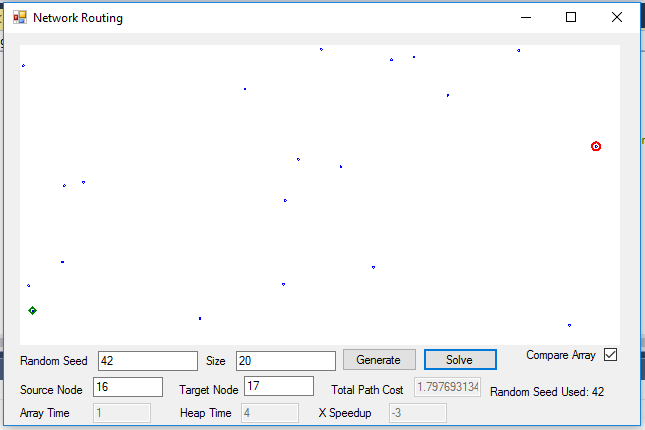
\includegraphics[resolution=72, width=\textwidth]{firstEx}
        \caption{20 points}
    \end{figure}
        \begin{figure}[p]
        \centering
        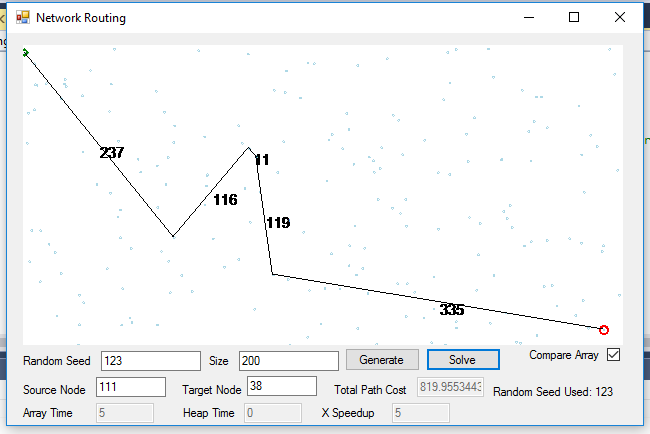
\includegraphics[resolution=72, width=\textwidth]{secEx}
        \caption{200 points}
    \end{figure}
    \item See table.  Didn't finish early enough (also computer too slow) to run 100,000 point tests.
    \begin{table}[]
\centering
\caption{Runtime differences, in milliseconds:}
\label{my-label}
\begin{tabular}{lllllll}
Nodes: & Run 1 & Run 2 & Run 3 & Run 4 & Run 5 & Average difference in ms \\
100    & 1     & 0     & 1     & 1     & 1     & .8                       \\
1000   & 75    & 80    & 85    & 72    & -3    & 61.8                     \\
10000  & 7261  & 7066  & 7357  & 7171  & 10242 & 7819                    
\end{tabular}
\end{table}
\end{itemize}
\end{document}


